\documentclass[11pt]{book}
\usepackage[subpreambles=true]{standalone}
\usepackage[spanish]{babel}
\usepackage{comfortaa}
\usepackage[T1]{fontenc}
\renewcommand*\oldstylenums[1]{{\firaoldstyle #1}}
\usepackage[T1]{fontenc}
\usepackage[utf8]{inputenc}
\usepackage[
letterpaper,
left=1in, 
right=1in, 
top=1in,
bottom=1in,
headheight=10mm,% Set \headheight to 10mm
]{geometry} % Custom margins
\usepackage{float}
\usepackage[colorlinks = true, linkcolor = blue]{hyperref}
\usepackage{bookmark}
\usepackage{fancyhdr}
\usepackage{color, colortbl}
\usepackage[dvipsnames,table]{xcolor} % Required for custom color
\usepackage{graphicx}
\usepackage{tabularx}
\usepackage{multicol,multirow}
\usepackage{newclude}
\usepackage{tabto}
\usepackage{remreset}
\usepackage[inline]{enumitem}
\usepackage{xparse}
\usepackage{wrapfig}
\usepackage{amssymb,amsmath}
\usepackage{tikz}
\usepackage{subfiles}
\usepackage{etoolbox}
\usepackage{subfiles} % Best loaded last in the preamble
\input{insbox}
\decimalpoint
%\captionsetup{width=.45\textwidth}
\setlength{\parindent}{0pt}
\graphicspath{{./Images}} %Setting the graphicspath
\definecolor{colorrds}{HTML}{0060A0} % Custom colour
%%% Headings and footer
\renewcommand\spanishtablename{Tabla}
\cfoot{\thepage}
\renewcommand{\headrulewidth}{0.2pt}
\renewcommand{\footrulewidth}{0.2pt}
%%%
\usetikzlibrary{
  arrows,
  positioning,
  matrix,
  calc,
  decorations.pathreplacing,
  decorations.pathmorphing,
  decorations.markings,
  decorations.text,
  shapes,
  backgrounds,
  shadows,
  trees,
  fit,
  snakes,
  patterns,
  mindmap,
  intersections,
  calendar,
  plotmarks,
  spy,
  tikzmark}

  \tikzset{
  abstractbox/.style={
    draw=black, fill=white, rectangle, 
    inner sep=12pt, style=rounded corners,
    drop shadow={fill=black, opacity=1}
  },
  abstracttitle/.style={fill=white}
}
%%%% APRENDISAJES TEXTBOX
\tikzset{
  abstractbox/.style={
    draw=black, fill=white, rectangle, 
    inner sep=15pt, style=rounded corners,
    drop shadow={fill=black, opacity=1}
  },
  abstracttitle/.style={fill=white}
}
\newcommand{\boxabstract}[2][fill=white]{
  \begin{tikzpicture}
    \node [abstractbox, #1] (box)
    {\begin{minipage}{0.9\linewidth}
        \setlength{\parindent}{0mm} % Indentar.
        \normalfont #2
      \end{minipage}};
    \node[abstracttitle, right=5pt] at (box.north west) {\textbf{Aprendizajes esperados:}};
    \node[draw=none, fit=(box)] {};
  \end{tikzpicture}
}%
%%%%%%%%%%%%%%%%%%%%%%%%

\makeatletter
  \@removefromreset{section}{chapter}
\makeatother
\addto\captionsspanish{\renewcommand{\chaptername}{Unidad}}
\renewcommand{\thechapter}{\arabic{chapter}}
\renewcommand{\thesection}{S\arabic{section}}
\renewcommand{\thesubsection}{L\arabic{subsection}}
\renewcommand{\labelenumi}{\mbox{\arabic{enumi}}}
\renewcommand{\labelitemi}{$\square$}

%%%%%%%%%%%%% START questions env
%Idea from https://tex.stackexchange.com/a/236668/1952
% \DeclareDocumentCommand\question{o}{%
%     \item\IfNoValueTF{#1}{}{(#1 puntos)}}
% \newenvironment{questions}[1][]{\enumerate[,#1]}{\endenumerate}
%\DeclareDocumentCommand\part{o}{%
% \item\IfNoValueTF{#1}{}{(#1 puntos)}}
% \newenvironment{parts}[1][]{\enumerate[,#1]}{\endenumerate}
% \newcommand{\part}{\item}
%%\newcommand{\choice}{\item}
% \newlist{parts}{enumerate*}{1}
% \setlist[parts,1]{label=(\alph*), itemjoin={{\quad}},leftmargin = 1cm}
% \newlist{oneparchoices}{enumerate*}{1}
% \setlist[oneparchoices,1]{label=\quad\alph*), itemjoin={{\quad}},leftmargin = 1cm}
% \newlist{choices}{itemize}{1}
% \setlist[choices,1]{label=\quad$\square$, itemjoin={{\\}},leftmargin = 1cm}
\newlist{hoptboxes}{itemize*}{1}
\setlist[hoptboxes,1]{label=\Large$\square$, font=\color{colorrds},itemjoin={{\quad}},leftmargin = 1cm}
\newlist{hoptions}{enumerate*}{1}
\setlist[hoptions,1]{label=(\alph*), font=\color{colorrds},itemjoin={{\quad}},leftmargin = 1cm}
%%%%%%%%%%%%% END questions env
\newenvironment{mybox}[3][]{%
  \begin{tikzpicture}[#1]%
    \def\myboxname{#3}%
    % good options: minimum height, minimum width
    \node [draw, inner sep=2ex,  align=justify]
      (BOXCONTENT) \bgroup\rule{0ex}{0ex}\ignorespaces
  }{%
    \egroup;
    \node [right, inner sep=3pt, fill=colorrds!75, outer sep=0pt, 
      text height=2ex, text depth=.5ex] (BOXNAME) 
      at ([shift={(-1em,5pt)}]BOXCONTENT.north west) {\myboxname};
    \fill[colorrds] (BOXNAME.north east) -- +(-1em,1em)
      -- +(-1em,0) -- cycle;
    \fill[colorrds] (BOXNAME.south west) -- +(1em,-1em)
      -- +(1em,0) -- cycle;
  \end{tikzpicture}
}
\begin{document}
\pagestyle{empty}
\newgeometry{left=0mm,top=50mm,bottom=0mm,right=0mm}
\documentclass[]{book}
\usepackage{geometry,graphicx} % Custom margins
\usepackage[spanish]{babel}
\usepackage[T1]{fontenc}
\usepackage[dvipsnames]{xcolor} % Required for custom color
\usepackage{color,colortbl}
\usepackage[utf8]{inputenc}
\usepackage{geometry} % Custom margins
\usepackage[spanish]{babel}
\usepackage{adjustbox,dashbox}
\usepackage{array}
\usepackage{tikz,pgfplots,pgfkeys}
\usepackage{forest,mathtools,siunitx}
\usepackage{amsfonts, amssymb, amsxtra, amsmath, amsbsy}
\usepackage{newclude}
\usepackage{ifthen}
\usepackage{float}
\usepackage{fancybox}
\usepackage{graphicx,tabularx}
\usepackage{multicol,multirow}
\usepackage{enumitem} % Customising the numbered lists
\usepackage{xhfill} % Making the pink block not extend beyond the margin
\usepackage{nameref} % reference the names of the sections
\usepackage{caption,capt-of}
\usepackage[normalem]{ulem} % Dashed lines in appendix
\usepackage{ragged2e} % Ragged left
\usepackage{booktabs}
\usepackage[unboxed]{cwpuzzle}
\usepackage[colorlinks = true,linkcolor = blue]{hyperref}
\usepackage{subfiles}
\usepackage{wrapfig}
\input{insbox}
\usepackage{etoolbox}
\usepackage{mwe}
\usepackage{comfortaa}
\usepackage[T1]{fontenc}
\renewcommand*\oldstylenums[1]{{\firaoldstyle #1}}
\usepackage[T1]{fontenc}
\usepackage{pythontex}
\usepackage{polynom}
\usepackage{longdivision}


\title{Actividades}
\author{Julio C. Melchor P.\thanks{{\tt julio.melchor@rafaeldiazserdan.net}}}
\date{v1.0, \today}
%\usepackage[dvipsnames]{xcolor} % Required for custom color
\usepackage{color,colortbl}
\usepackage[utf8]{inputenc}
\usepackage{geometry} % Custom margins
\usepackage[spanish]{babel}
\usepackage{adjustbox,dashbox}
\usepackage{array}
\usepackage{tikz,pgfplots,pgfkeys}
\usepackage{forest,mathtools,siunitx}
\usepackage{amsfonts, amssymb, amsxtra, amsmath, amsbsy}
\usepackage{newclude}
\usepackage{ifthen}
\usepackage{float}
\usepackage{fancybox}
\usepackage{graphicx,tabularx}
\usepackage{multicol,multirow}
\usepackage{enumitem} % Customising the numbered lists
\usepackage{xhfill} % Making the pink block not extend beyond the margin
\usepackage{nameref} % reference the names of the sections
\usepackage{caption,capt-of}
\usepackage[normalem]{ulem} % Dashed lines in appendix
\usepackage{ragged2e} % Ragged left
\usepackage{booktabs}
\usepackage[unboxed]{cwpuzzle}
\usepackage[colorlinks = true,linkcolor = blue]{hyperref}
\usepackage{subfiles}
\usepackage{wrapfig}
\input{insbox}
\usepackage{etoolbox}
\usepackage{mwe}
\usepackage{comfortaa}
\usepackage[T1]{fontenc}
\renewcommand*\oldstylenums[1]{{\firaoldstyle #1}}
\usepackage[T1]{fontenc}
\usepackage{pythontex}
\usepackage{polynom}
\usepackage{longdivision}

 % Imports all the required packages. See Functional/%Packages.tex for more detailS
\geometry{letterpaper,total={175mm,220mm},left=15mm,top=50mm,bottom=0mm} % Custom margins

\begin{document}
\pagestyle{empty}
\begin{center}
    {\Huge Matem\'aticas 3}\\
    \vspace{1cm}
    \normalsize
    \textbf{\large Cuaderno de trabajo}\\
    para los alumnos de 3$^\circ$ de  Secundaria\\
    en el curso durante el ciclo escolar\\
    \textbf{2022-2023}\\
    \vspace{2.2cm}
    \small POR\\
    \Large J. C. Melchor Pinto\\[0.5em]
    \normalsize Profesor de asignatura en\\
    \vspace{1cm}
    
\includegraphics[width=5cm]{../Unidad 2/Images/LOGO_RDS_nobg}
\end{center}
\vspace{2.5cm}
%\include*{Functional/TitlePage}
\hspace{-16mm}

\includegraphics[width=\paperwidth]{../Unidad 2/Images/cover_bg}
\end{document}

\restoregeometry
\tableofcontents
\chapter{}
\pagestyle{fancy}
\section{Multiplicación de fracciones y decimales positivos}
\subsection{Multiplicación de fracciones y decimales}

\section{Multiplicación y división con fracciones y decimales positivos}
\subsection{División con números fraccionarios}
\subsection{Problemas de multiplicación y división de fracciones}

\section{Multiplicación y división de números positivos y negativos}
\subsection{Multiplicación de números positivos y negativos}
\subsection{División de números positivos y negativos}
\subsection{Multiplicación y división de números con signo}

\section{Potencia con exponente entero}
\subsection{Productos de potencias enteras de la misma base}
\subsection{Potencia de una potencia entera}
\subsection{Cociente de potencias enteras de la misma base}
\subsection{Potencias con exponente negativo y notación científica}

\section{Raíces cuadradas}
\subsection{Significado de la raíz cuadrada}
\subsection{Aproximación de raíces cuadradas}
\subsection{Cuadrados y raíces cuadradas}

\section{Propiedades de polígonos}
\subsection{Diagonales de un polígono}
\subsection{Ángulos de un polígono}

\section{Construcción de polígonos regulares}
\subsection{Algunas construcciones de polígonos}

\section{Conversión de unidades del SI y del sistema inglés}
\subsection{Conversión entre unidades del SI}
\subsection{Conversión entre unidades del sistema inglés}
\subsection{Conversión de unidades del SI al sistema inglés y viceversa}

\section{Histogramas, polígonos de frecuencias y gráficas de línea}
\subsection{Histogramas}
\subsection{Polígonos de frecuencias}
\subsection{Gráficas de línea}
\subsection{Elección de la representación gráfica más adecuada}

\chapter{}

\section{Proporcionalidad directa e inversa}
\boxabstract{Resuelve problemas de proporcionalidad directa e inversa y de reparto proporcional}
\subsection{Proporcionalidad directa e inversa}
\begin{minipage}{0.45\textwidth}
  \begin{mybox}{0.45\linewidth}{
      \begin{comfortaa}
        \color{white}Definici\'on
      \end{comfortaa}}
    \begin{minipage}{0.90\linewidth}
      \textbf{Proporcionalidad Directa:}\\ Relaci\'on entre dos cantidades que cambian en el mismo sentido.
    \end{minipage}%
  \end{mybox}
\end{minipage}\hfill
\begin{minipage}{0.45\textwidth}
  \begin{mybox}{0.45\linewidth}{
      \begin{comfortaa}
        \color{white}Definici\'on
      \end{comfortaa}}
    \begin{minipage}{0.90\linewidth}
      \textbf{Proporcionalidad Inversa:}\\ Relaci\'on entre dos cantidades que cambian en sentidos opuestos.
    \end{minipage}%
  \end{mybox}
\end{minipage}%

% Dos magnitudes son directamente proporcionales si al multiplicar (o dividir) una de ellas por un número, la otra queda
% multiplicada (o dividida) por el mismo número. El cociente entre la segunda y la primera magnitud es constante y se
% denomina constante de proporcionalidad directa.

% Dos cantidades son inversamente proporcionales si al multiplicar (o dividir) una de ellas por un número la otra
% queda dividida (o multiplicada) por el mismo número. El producto de la segunda y la primera magnitud es constante
% y se llama constante de proporcionalidad inversa.

\begin{enumerate}
  \item Señala si las relaciones son directamente proporcionales o inversamente proporcionales.
        %   \begin{multicols}{2}
        %\NumTabs{2}
        \begin{enumerate}
          \item La población mundial y el consumo de agua.\\
                \begin{hoptboxes}%[label=$\square$,font=\color{colorrds},itemjoin={\qquad}]
                  \item Directamente proporcional
                  \item Inversamente proporcional
                \end{hoptboxes}
          \item  La población mundial y la cantidad de agua disponible por persona.\\
                \begin{hoptboxes}%[label=$\square$,font=\color{colorrds},itemjoin={\qquad}]
                  \item Directamente proporcional
                  \item Inversamente proporcional
                \end{hoptboxes}
          \item La distancia al sol y la temperatura.\\
                \begin{hoptboxes}%[label=$\square$,font=\color{colorrds},itemjoin={\qquad}]
                  \item Directamente proporcional
                  \item Inversamente proporcional
                \end{hoptboxes}
          \item  El tamaño de un planeta y su fuerza de gravedad.\\
                \begin{hoptboxes}%[label=$\square$,font=\color{colorrds},itemjoin={\qquad}]
                  \item Directamente proporcional
                  \item Inversamente proporcional
                \end{hoptboxes}
          \item  La velocidad de un móvil y la distancia recorrida.\\
                \begin{hoptboxes}%[label=$\square$,font=\color{colorrds},itemjoin={\qquad}]
                  \item Directamente proporcional
                  \item Inversamente proporcional
                \end{hoptboxes}
          \item La cantidad de imágenes guardadas en el celular y la cantidad de espacio libre.\\
                \begin{hoptboxes}%[label=$\square$,font=\color{colorrds},itemjoin={\qquad}]
                  \item Directamente proporcional
                  \item Inversamente proporcional
                \end{hoptboxes}
          \item  El tamaño de un archivo y el tiempo de descarga.\\
                \begin{hoptboxes}%[label=$\square$,font=\color{colorrds},itemjoin={\qquad}]
                  \item Directamente proporcional
                  \item Inversamente proporcional
                \end{hoptboxes}
          \item La velocidad de conexión a Internet y el tiempo de descarga de archivos.\\
                \begin{hoptboxes}%[label=$\square$,font=\color{colorrds},itemjoin={\qquad}]
                  \item Directamente proporcional
                  \item Inversamente proporcional
                \end{hoptboxes}
        \end{enumerate}
        %  \end{multicols}

\end{enumerate}
\subsubsection{Proporcionalidad con tablas de variación}
Para identificar las características de los tipos de relaciones, en
especial las que se refieren a proporcionalidad inversa, Analiza las siguientes situaciones, completa las tablas
de variaci\'on y responde a cada una de las preguntas.

\begin{enumerate}
  \item La autopista 10 en Haradh, Arabia Saudita, tiene más de 200
        km en línea recta. Un automóvil viaja por esta carretera con
        velocidad constante de 120 km/h durante 200 km.
        \begin{table}[!h]
          \centering
          \begin{tabular}{|c|c|}
            \hline
            Distancia [km] & Tiempo [h] \\
            \hline\rowcolor{colorrds!20}
            50             &            \\
            \hline
            75             &            \\
            \hline\rowcolor{colorrds!20}
            100            &            \\
            \hline
            125            &            \\
            \hline\rowcolor{colorrds!20}
            150            &            \\
            \hline
            175            &            \\
            \hline\rowcolor{colorrds!20}
            200            &            \\
            \hline
          \end{tabular}
          \caption{}
          \label{table:arabia}
        \end{table}
        \begin{enumerate}
          \item Completen la Tabla \ref{table:arabia} que registra la velocidad del automóvil.
          \item ¿Cómo es la variación de los datos de la tabla? ¿Por qué?
          \item ¿En cuántos minutos recorre 1 km? Explica tu procedimiento.
          \item ¿En cuánto tiempo se recorrieron 120 km? ¿Y en cuánto tiempo se recorrerán 230 km?
        \end{enumerate}

  \item Analicen los rectángulos de la figura 2.1. La tabla \ref{table:rectangulos} muestra las medidas de los lados de cada uno. Complétenla.
        \begin{figure}[H]
          \centering
          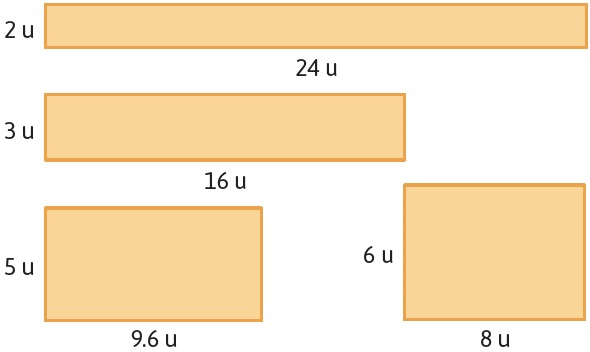
\includegraphics[width=0.7\textwidth]{ejem10.2}
        \end{figure}

        \begin{table}[!h]
          \centering
          \begin{tabular}{|l|c|c|c|}
            \hline
                         & Lado 1 (u) & Lado 2 (u) & Área (u$^2$) \\
            \hline
            Rectángulo 1 & 2          & 24         & 48           \\
            Rectángulo 2 & 3          &            &              \\
            Rectángulo 3 & 5          &            &              \\
            Rectángulo 4 & 6          &            &              \\
            \hline
          \end{tabular}
          \caption{}
          \label{table:rectangulos}
        \end{table}
        \begin{enumerate}
          \item Completa la Tabla \ref{table:rectangulos} que muestra la medida de los lados de un conjunto de rect\'angulos.
          \item ¿Cómo es la variación de los datos de la tabla? ¿Por qué?
          \item Si se añade el rectángulo cuyo lado 1 mide 4 u, ¿cuál es la medida del otro lado? ¿Cuál es su área? Expliquen su procedimiento.
          \item ¿Cómo es el área de los rectángulos?
        \end{enumerate}
\end{enumerate}



\subsection{Problemas sobre proporcionalidad directa e inversa}

Presentamos diversas situaciones que involucran la interpretación de relaciones directas e inversas.
Intenta resolver por tu cuenta cada situación. Luego, una vez que agotes todas tus estrategias, analiza con detenimiento las propuesta de resolución de cada situación.

\subsubsection{Ejemplo 1}

Marcos sale diariamente con su bicicleta y recorre todo el contorno del parque de su barrio. Él sabe que tarda aproximadamente 6 minutos en dar 3 vueltas al parque.
Si Marcos quiere dar 12 vueltas al parque,
\textbf{¿cuánto tiempo tardará?}\\

Asignemos $x$ a la cantidad de vueltas e $y$ el tiempo necesario para dar las $x$ vueltas.

\begin{center}
  $x$ = n\'umero de vueltas. \quad $y$ = tiempo para dar las vueltas.
\end{center}
Planteamos la relación directa entre $x$ e $y$.
\[y=kx\]
Reemplazamos los valores que nos dan en la situación; 6 minutos para dar 3 vueltas. Es decir, $x=3$ e $y=6$.
\[6=k(3) \Rightarrow k=2\]
Por tanto, la relación proporcional es $y=2x$.
Como nos piden calcular la cantidad de minutos que necesita Marcos para dar 12 vueltas, sabemos que $x=12$.
Reemplazamos:
\[y=2(12) \Rightarrow y=24\]
Por tanto, Marcos tardará 24 minutos en dar 12 vueltas alrededor del parque de su barrio.
\subsubsection{Ejemplo 2}
Cinthia va a la escuela en bicicleta desde su casa. Ella calcula que llega al colegio en 45 minutos cuando va a una velocidad promedio de 0.75 kilómetros por minuto.
\textbf{¿Cuánto tiempo tardará si cambia la velocidad a 0.5 kilómetros por minuto?}

Asignemos $t$ al tiempo que demora en ir de su casa a la escuela y $v$ a la velocidad promedio de su bicicleta.
\begin{center}
  $t$ = tiempo. \quad $v$ = velocidad.
\end{center}
Observa que la relación entre el tiempo y la velocidad es una relación inversa. Planteamos esa relación inversa entre $x$ e $y$.
\[v=k \times \frac{1}{t}\]
Reemplazamos los valores que nos dan en la situación, 45 minutos a una velocidad de 0.75 kilómetros por minuto. Es decir $x=45$ e $y=0.75$.
\[0.75=k\times \frac{1}{45} \Rightarrow k=33.75\]
Por tanto, la relación proporcional es:
\[v=33.75 \times \frac{1}{t}\]
Como nos piden calcular la cantidad de minutos que tarda en llegar a la escuela a una velocidad de 0.5 kilómetros por minuto, sabemos que \[0.5=33.75 \times \frac{1}{t} \Rightarrow t=67.5 \text{ minutos}\]
Por tanto, Cinthia tardará 67.5 minutos en llegar a la escuela a una velocidad de 0.5 kilómetros por minuto.

\subsubsection{Ejemplo 3}

En una tienda se venden rollos de papel higiénico. Cada rollo cuesta 2 dólares, pero hay la siguiente oferta:
Lleva 3 rollos de papel higiénico y paga solo 2.
Carlos compra 20 rollos del papel higiénico en oferta en esa tienda.\\
\textbf{¿Es correcto afirmar que pagó 40 dólares?}\\

Para resolver este problema utilizaremos una tabla de valores como la siguiente:


% \begin{tikzpicture}
%   \matrix[matrix of math nodes,draw, column sep=1em,row sep=.5mm] (mx) {
%     3 & 2 & $2\times2=4 $ \\
%     4 & 3 & $2\times3=6 $ \\
%     5 & 4 & $2\times4=8 $ \\
%     6 & 4 & $2\times4=8 $ \\
%     7 & 5 & $2\times5=10$ \\
%     8 & 6 & $2\times6=12$ \\
%     9 & 6 & $2\times6=12$ \\
%   };
%   \path[->,shorten >=2pt]
%   \foreach \from/\to in {1/9} {
%       ([yshift=2mm]mx-1-\from.north) edge[bend left]
%       node[above] {$\scriptstyle+1$} ([yshift=2mm]mx-1-\to.north)
%       ([yshift=-2.5mm]mx-2-\from.south) edge[bend right]
%       node[below] {$\scriptstyle+2$} ([yshift=-2.5mm]mx-2-\to.south)
%     };
%   \foreach \x in {2,...,6}{
%       \draw ([xshift=-0.5em]mx.north west -| mx-1-\x.west) -- ([xshift=-0.5em]mx.south west -| mx-1-\x.west);
%     };
%   \draw (mx.west) -- (mx.east);
% \end{tikzpicture}
% % \end{table}


\begin{figure}[H]
  \centering
  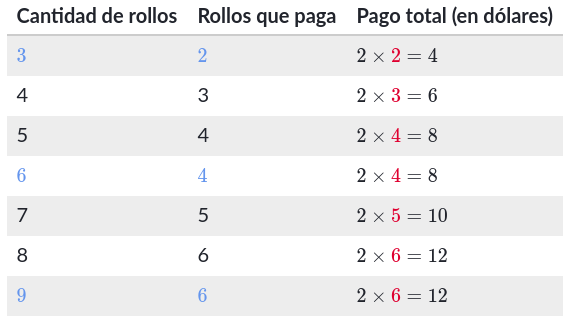
\includegraphics[width=0.7\textwidth]{./Unidad 2/Images/tableS8L102.png}
\end{figure}

Observamos que, si la cantidad de rollos es un múltiplo de 3, se cumple una relación proporcional directa entre dicha cantidad y los rollos que deberá pagar.\\

Como Carlos compra 20 rollos, podemos observar que el múltiplo de 3 más cercano a 20 es 18. Así obtendremos la cantidad de rollos a pagar luego de aplicar la oferta.\\

\begin{figure}[H]
  \centering
  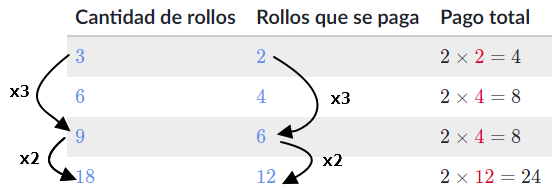
\includegraphics[width=0.5\textwidth]{./Unidad 2/Images/tableS8L101.png}
\end{figure}

Gracias a la tabla, podemos observar que, llevando 18 rollos en oferta, solo pagará 12 rollos, es decir, 24 dólares. Para comprar los 20 rollos, Carlos deberá pagar 2 rollos adicionales a un monto de 4 dólares.\\

Finalmente, por toda la compra pagará 24 dólares más 4 dólares adicionales, es decir, un total de 28 dólares.\\

Por tanto, la afirmación no es correcta. Carlos no pagó 40 dólares, sino 28.

\subsubsection{Ejemplo 4}
Un grupo de 64 obreros puede terminar una obra en 15 días. Al cabo de 5 días de trabajo, se les unen obreros de otro grupo, de modo que tardan 5 días menos en terminar la obra.\\
\textbf{¿Cuántos obreros había en el segundo grupo?}\\

Sabemos que 64 obreros terminarían la obra en 15 días. Como luego de los primeros 5 días de trabajo llegaron más obreros, hacemos el siguiente gráfico para representar la situación:
\begin{figure}[H]
  \centering
  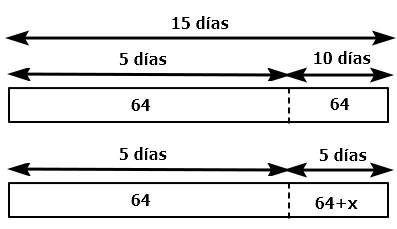
\includegraphics[width=0.5\textwidth]{./Unidad 2/Images/tableS8L103.png}
\end{figure}
Observamos que, en esta situación, a mayor cantidad de obreros, menos días se necesitarán para terminar la obra.\\

\begin{table}[H]
  \centering
  \begin{tabular}{|l|c|l|}
    \hline
    Cantidad de obreros         & 64 & 64+x \\
    \hline
    Cantidad de días de trabajo & 10 & 5    \\
    \hline
  \end{tabular}
\end{table}

Como es una relación inversamente proporcional, planteamos la siguiente relación:
\begin{align*}
  64 \times 10 & = 5 \times (64+x) \\
  640          & = 320 +5x         \\
  5x           & = 320             \\
  x            & = 64
\end{align*}

En el segundo grupo, había 64 obreros más, es decir, un total de 128 obreros.


\newpage
\subsubsection{Ejercicios}
Copia en tu libreta los siguientes problemas. Realiza para cada uno de ellos todas las operaciones y
procedimientos necesarios para obtener la respuesta a cada una de las preguntas. Al terminar, señala la
opción que contenga la respuesta correcta.
\begin{enumerate}%[start=1]%<--- start option fixes number for first item
  \item Un grupo de 20 obreros puede terminar una
        construcción en 40 días. Al cabo de 10 días de trabajo,
        se les unen obreros de otro grupo, de modo que en 15 días
        más terminan la obra.\\
        \textbf{¿Cuántos obreros había en el segundo grupo?}\\
        \emph{Escoge 1 respuesta:}\\
        \begin{hoptions}
          \item 20 obreros
          \item 5 obreros
          \item 10 obreros
          \item 15 obreros
        \end{hoptions}

  \item Mateo va en auto de su casa a la universidad. Si va a una velocidad promedio de 60 kilómetros por hora, tarda 1 hora.\\
        \textbf{¿Cuánto tiempo tardaría si fuera a 40 kilómetros por hora?}\\
        \emph{Escoge 1 respuesta:}\\
        \begin{hoptions}
          \item 1 hora y 30 minutos
          \item 30 minutos
          \item 1 hora y 20 minutos
          \item 2 horas
        \end{hoptions}

  \item En una tienda, se venden rollos de papel higiénico. Cada rollo cuesta 2 dólares, pero hay la siguiente oferta:
        Lleva 3 rollos de papel higiénico y paga s\'olo 2.
        María va a la tienda a comprar 20 rollos de papel higiénico en oferta.\\
        \textbf{¿Cuánto pagará por la compra?}\\
        \emph{Escoge 1 respuesta:}\\
        \begin{hoptions}
          \item 28 dólares
          \item 17 dólares
          \item 30 dólares
          \item 14 dólares
        \end{hoptions}

  \item Un grupo de 32 tejedores puede terminar un pedido de ponchos en 15 días. Al cabo de 5 días de trabajo, se les unen tejedores de otro grupo, de modo que en 8 días más terminan el pedido.\\
        \textbf{¿Cuántos tejedores había en el segundo grupo?}\\
        \emph{Escoge 1 respuesta:}\\
        \begin{hoptions}
          \item 8 tejedores
          \item 16 tejedores
          \item 32 tejedores
          \item 10 tejedores
        \end{hoptions}

  \item \textbf{¿Cuál ecuación muestra variación directa?}\\
        \emph{Escoge 1 respuesta:}\\
        \begin{hoptions}
          \item $\dfrac{1}{5}\cdot a=\dfrac{1}{b}$
          \item $a\cdot b=\dfrac{1}{5}$
          \item $a=5\cdot \dfrac{1}{b}$
          \item $\dfrac{a}{b}=5$
          \item $a\cdot b=5$
        \end{hoptions}

  \item \textbf{¿Cuál ecuación muestra variación inversa?}\\
        \emph{Escoge 1 respuesta:}\\
        \begin{hoptions}
          \item $2\cdot \dfrac{1}{a}=\dfrac{1}{b}$
          \item $\dfrac{1}{2}\cdot \dfrac{1}{a}=\dfrac{1}{b}$
          \item $2\cdot a=b$
          \item $\dfrac{a}{b}=\dfrac{1}{2}$
          \item $a\cdot b=2$
        \end{hoptions}

  \item En el mercado, 2 kilogramos de papa cuestan \$3.5 dólares.
        Sofía tiene \$25 dólares para comprar 14 kilogramos de papa.\\
        \textbf{¿Cuáles de las siguientes afirmaciones son correctas?}\\
        \emph{Elige todas las respuestas adecuadas:}\\
        \begin{hoptboxes}
          \item Deberá pagar \$7.5 dólares por 6 kilogramos de papa.\\
          \item Pagará \$14 dólares por 8 kilogramos de papa.\\
          \item Sofía recibirá \$0.50 dólares de vuelto.\\
          \item Sofía necesitará más dinero para realizar la compra.\\
        \end{hoptboxes}

\end{enumerate}

\newpage
\subsubsection{Problemas}

\begin{enumerate}
  \item Estás preparando limonada. La cantidad de azúcar que necesitas depende de la cantidad de limones que uses,
        como se muestra en la tabla \ref{table:azucar_limon}.
        \begin{table}[!h]
          \centering
          \begin{tabular}{|l|c|c|c|}
            \hline
            Tazas de azúcar     & $\frac{1}{3}$ & 1 & 3 \\
            \hline
            Cantidad de limones & 1             & 3 & 9 \\
            \hline
          \end{tabular}
          \caption{}
          \label{table:azucar_limon}
        \end{table}\\
        \textbf{¿Cuál es la constante de proporcionalidad entre las tazas de azúcar y los limones?}

  \item Un carpintero fabrica sillas, las cuales le cuestan \$250.00 elaborar
        cada una. Además, tiene costos fijos por la renta del local y equi-
        po que es de \$3 500.00 al mes. \\
        \textbf{¿Cuántas sillas hacen que el precio por producirlas sea igual a los costos fijos?}\\

  \item El equipo conformado por Cristina, Javier y Claudia tardó 8 días en responder 120 preguntas que su profesor de Historia de México les dejó de tarea.
        \begin{enumerate}
          \item ¿Cuántas preguntas resolvieron Cristina, Javier y Claudia cada día?
                \begin{hoptions}
                  \item 3 preguntas \item 5 preguntas \item 8 preguntas \item 15 preguntas
                \end{hoptions}
          \item ¿Cuántas preguntas respondió cada uno de los integrantes del equipo por día?
                \begin{hoptions}
                  \item 3 preguntas \item 5 preguntas \item 8 preguntas \item 15 preguntas
                \end{hoptions}
          \item Si el equipo estuviera formado por 5 personas, ¿cuántas preguntas respondería cada una en un solo día, suponiendo que trabajan al mismo ritmo?
                \begin{hoptions}
                  \item 3 preguntas \item 5 preguntas \item 8 preguntas \item 15 preguntas
                \end{hoptions}
          \item ¿En cuántos días responderían las 120 preguntas si el equipo estuviera formado por 8 personas, suponiendo que trabajan al mismo ritmo que el equipo original?
                \begin{hoptions}
                  \item 3 días \item 5 días \item 8 días \item 15 días
                \end{hoptions}
          \item Si sólo hubieran sido 45 preguntas y el equipo estuviera formado por 5 personas que trabajan al mismo ritmo, ¿en cuantos días terminarían la tarea?
                \begin{hoptions}
                  \item 2 días \item 5 días \item 8 días \item 15 días
                \end{hoptions}
        \end{enumerate}

  \item Tania tiene 5 parejas de canarios y necesita 15 paquetes de comida para alimentarlos durante 30 días.
        \begin{enumerate}
          \item ¿Cuántos días podría alimentar a los canarios con un paquete de comida?\\
                \begin{hoptions}
                  \item  5 días
                  \item 10 días
                  \item 30 días
                  \item 90 días
                \end{hoptions}
          \item ¿Cuántos días podría alimentar a los canarios con el triple de alimento?\\
                \begin{hoptions}
                  \item 1 día
                  \item 2 días
                  \item 3 días
                  \item 5 días
                \end{hoptions}
          \item ¿Cuántos días le durarían los 15 paquetes de comida para alimentar al triple de canarios?\\
                \begin{hoptions}
                  \item 15 días
                  \item 30 días
                  \item 60 días
                  \item 90 días
                \end{hoptions}
          \item Si Tania tuviera un total de 10 parejas de canarios, ¿cuántos días podría alimentarlos con un
                solo paquete de comida?\\
                \begin{hoptions}
                  \item 5 días
                  \item 10 días
                  \item 30 días
                  \item 90 días
                \end{hoptions}
          \item Si Tania tuviera 30 canarios, ¿cuántos días le durarían 5 paquetes de comida?\\
                \begin{hoptions}
                  \item  1 día
                  \item 2 días
                  \item 3 días
                  \item 5 días
                \end{hoptions}
        \end{enumerate}
\end{enumerate}
\section{Reparto Proporcional}
\subsection{Situaciones de reparto proporcional}

\section{Sistemas de ecuaciones lineales con dos inc\'ognitas}
\subsection{Ecuaciones lineales}
\subsection{Sistemas de ecuaciones lineales con dos inc\'ognitas}

\section{M\'etodos algebraicos de soluci\'on de sistemas de ecuaciones}
\subsection{Soluci\'on de sistemas de ecuaciones}
\subsection{Problemas sobre sistemas de ecuaciones lineales}

\section{Variabilidad lineal y proporcionalidad inversa}
\subsection{Situiaciones de variación lineal}
\subsection{Representaciones de proporcionalidad inversa}

\section{Modelos de variación lineal y proporcionalidad inversa}
\subsection{Modelos de variación lineal y proporcionalidad inversa}

\section{Per\'imetro y \'area de pol\'igonos regulares}
\subsection{Per\'imetro y \'area de pol\'igonos}

\section{\'Area del c\'irculo}


\subsection{Area del c\'irculo}
El área de un círculo es la cantidad de espacio que abarca. También podemos pensarla como la cantidad total de espacio dentro del círculo.
Para encontrar el área de un círculo podemos utilizar la siguiente fórmula:
\[A=\pi r^2\]

\subsubsection{Ejemplo 1: encontrar el área, dado el radio}
Encuentra el área de un círculo de radio 5.
\begin{figure}[H]
  \centering
  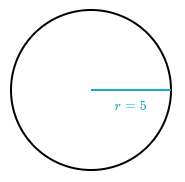
\includegraphics[width=0.5\textwidth]{./Unidad 2/Images/figS10_001.png}
\end{figure}
La ecuación para el área de un círculo es:
\begin{align*}
  A & = \pi r^2    \\
  A & = \pi 5^2    \\
  A & = \pi r^{25}
\end{align*}

Podemos detenernos aquí y escribir la respuesta como $25\pi$. O bien, podemos sustituir 3.14 por $\pi$ y multiplicar.\\
$A = 3.14 \cdot 25$\\
$A = 78.5$ unidades cuadradas\\
El área del círculo es $25\pi$ unidades cuadradas, o sea 78.5 unidades cuadradas.
\subsubsection{Ejemplo 2: encontrar el área, dado el diámetro}
Encuentra el área de un círculo de diámetro 16.
\begin{figure}[H]
  \centering
  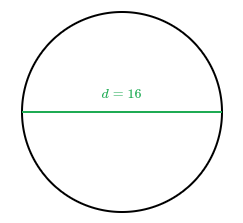
\includegraphics[width=0.5\textwidth]{./Unidad 2/Images/figS10_002.png}
\end{figure}
Primero encontremos el radio:

\begin{align*}
  r & = \dfrac d2     \\
  r & = \dfrac{16}{2} \\
  r & = 8
\end{align*}

Ahora podemos encontrar el área.\\

La ecuación para el área de un círculo es:
\begin{align*}
  A & = \pi r^2      \\
  A & = \pi \cdot 8  \\
  A & = \pi \cdot 64 \\
\end{align*}
Podemos detenernos aquí y escribir la respuesta como $64\pi$. O bien, podemos sustituir 3.14 por $\pi$ y multiplicar.\\
$A = 3.14 \cdot 64$\\
$A = 200.96$ unidades cuadradas\\

El área del círculo es $64\pi$ unidades cuadradas, o sea 200.96 unidades cuadradas.

\section{Medidas de tendencia central, rango y desviación media}
\subsection{Medidas de tendencia central}
\subsection{Rango y dispersi\'on de datos}
\subsection{Desviaci\'on media}


%%% U3
\chapter{}

\section{Sucesiones y equivalencia de expresiones}
\subsection{Reglas aritméticas y equivalencias}

\section{Figuras geométricas y equivalencia de expresiones}
\subsection{Equivalencia de expresiones algebraicas}
\subsection{Expresiones de perímetros y áreas}

\section{Volumen de prismas rectos}
\subsection{Volumen de primas rectos con base en forma de polígono regular}
\subsection{Problemas de volumen de prismas rectos}

\section{Volumen de cilindros rectos}
\subsection{Volumen de cilindros rectos}
\subsection{Problemas de cilindros rectos}

\section{Desarrollos planos de prismas y cilindros rectos}
\subsection{Desarrollos planos}

\section{Probabilidad teórica}
\subsection{Definición de probabilidad teórica}
\subsection{Probabilidad teórica y frecuencial}

\end{document}